\chapter{Applications}\label{ch:applications}

In this chapter, we describe how we use PINNs in the case of the models presented in Chapter~\ref{ch:galaxies-theory}. In particular, we detail the way in which the training points are generated, and present the results obtained for each of the models. More details are given on the hyperparameters, especially in section~\ref{sec:disk}, where the results of a fine-tuning of the hyperparameters for the exponential thick disk are presented.

\section{Hernquist Model}\label{sec:hernquist}

Firstly, we focus on the Hernquist model~\cite{hernquist_analytical_1990}, a simple model through which we aim to test the capability of a PINN in finding the solution $\hat{\Phi}$ of Equation~\eqref{eq:residual_poisson_hernquist1}. Specifically, we observe the training time and the highest accuracy reached by it.

\subsubsection{Theory}

We recall the differential equation~\eqref{eq:residual_poisson_hernquist1} that we aim to solve:

\begin{equation}
    \dfrac{\dd}{\dd s}\left(s^2 \dfrac{\dd \Phi'}{\dd s}\right) = \dfrac{2s}{(s+1)^3}
\end{equation} By utilizing this equation, along with the definition of the error function~\eqref{eq:loss-galaxy}, we can formulate the error function used to train the PINN to ascertain the Hernquist potential~\eqref{eq:hernquist_pot}:

\begin{equation}
    \mathcal{L}_(\theta) = \dfrac{1}{N_c}\sum^{N_c}_{i=1} \left|\dfrac{\dd}{\dd s_i}\left(s_{i}^{2} \dfrac{\dd \Phi'}{\dd s_i}\right) - \dfrac{2s_i}{(s_i+1)^3} \right|^2 + \dfrac{1}{N_d}\sum^{N_d}_{i=1} \left|\hat{\Phi}(s_i) - \Phi_i \right|^2
\end{equation}

For instance, this error function can be simply written\footnotemark using the PyTorch library~\cite{NEURIPS2019_9015}:
\begin{minted}{Python}
    def pde_residual(net, x):
        phi_pred = net(x)
        phi_x = torch.autograd.grad(phi_pred, x)[0]
        phi_x *= x ** 2
        df = torch.autograd.grad(phi_x, x)[0]
        residual = df - 2 * x / (x + 1) ** 3
        return residual.pow(2).mean()

    def boundary_error(net, x_b, y_true):
        phi_pred = net(x_b)
        error = y_true - phi_pred
        return error.pow(2).mean()

    def loss_function(net, x, x_b, y_true):
        return pde_residual(net, x) + boundary_error(net, x_b, y_true)

\end{minted}
\footnotetext{For readability, the illustrated code above omits certain arguments. For a complete implementation, please refer to the associated GitHub repository.}

\subsubsection{Training Points}

In order to train the model, we need to provide training points. In the case of the Hernquist model, we aim to generate points along the radial axis as $s$ is the only parameter of the function~\eqref{eq:hernquist_pot}. We also recall that we consider isolated systems for which $\Phi \to 0$ when $s \to \infty$. We want to study the potential from its origin, at $s=0$, up to a sufficiently large $s$ value such that $\Phi \simeq 0$. Therefore, the integration domain should be a line bounded on the left by $s_0 = 0$ and on the right by $s_n$ such that $\Phi(s_n) \simeq 0$. We now need to determine a suitable value for $s_n$.
\par If we set $|\Phi(s_n)| = \varepsilon$, and considering~\eqref{eq:hernquist_pot} we then have:

\begin{align*}
\label{eq:final-value-hernquist}
    |\Phi(s_n)| &= \frac{1}{s_n + 1} = \varepsilon \\
    \Rightarrow s_n &= \frac{1 - \varepsilon}{\varepsilon}
\end{align*} In our study, we consider that $\varepsilon = 10^{-3}$ is sufficiently close to $0$. This gives us a value of $s_n=999$, which we will simply round to $10^3$.

Given that the training domain is a line, we are limited to two data points, one at each end. In other words, $N_d = 2$ in equation~\eqref{eq:loss-func-hernquist}. As for the number of collocation points, $N_c$, the choice is free. Naturally, the computation time grows with $N_c$. We need enough points for accurate prediction, but not too many, to keep the computation time reasonable. Various values have been tested, but the results presented here were obtained for $N_c = 1024$. The configuration of the training points is illustrated in Figure~\ref{fig:training-points-hernquist}. The points are selected via the Latin Hypercube Sampling (LHS) algorithm (see Appendix~\ref{app:lhs}). 

Depending on the context, a neural network may tend to overfit, i.e., it conforms strictly to the presented data, thus losing its ability to generalize a result to new data. One way to check whether a network is not suffering from this issue is to monitor the error made on new data. This process first takes place during training, where the error on so-called \emph{validation} data is calculated at each epoch. Subsequently, the network's predictions are checked on other new, so-called \emph{test}, data. For our PINNs, these new data are domain points that the network has not seen during training. For the training data, we generate $N_c / 3$ points randomly distributed uniformly across the training domain. For the test data, we can take any interval included in the training interval.

\begin{figure}
    \centering
    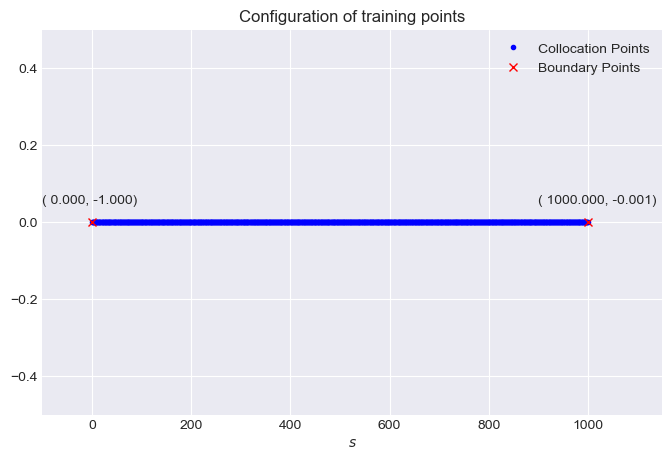
\includegraphics[width=\textwidth]{imgs/training-points-hernquist.png}
    \caption{Configuration of training points in the spatial domain $s \in [0, 1000]$. In red, the border points with their detailed coordinates $(s_0, \Phi(s_0))$. In blue, the $1024$ collocation points chosen via the Latin hypercube sampling algorithm. Although indiscernible on the graph, the points are on average spaced about $1000/1024 \approx 0.97$ length units apart. Note that the $y$ axis in this graph is purely illustrative and has no tangible reality.}
\label{fig:training-points-hernquist}
\end{figure}

\subsubsection{Training}

For training, we have several hyperparameter choices to make; the network architecture, the optimization function, the learning rate, and the number of epochs. Given the relatively simple expression of the potential, we choose a "light" architecture with 2 hidden layers and 32 neurons per layer. Numerous other architectures with more hidden layers and neurons were tested, but none provided results as good as those with 32 neurons. Keeping 32 neurons per layer and increasing the number of layers does not significantly improve accuracy, but it does substantially increase computation time. Furthermore, the L-BFGS optimizer performs poorly in our case in terms of convergence speed and accuracy.

Finally, the training was performed on a PINN with 2 hidden layers, each containing 32 neurons, with an Adam optimizer and an initial learning rate of $10^{-5}$. The term 'initial' is used because we employ a \emph{scheduler}. The scheduler's role is to modify the learning rate if the error function hits a plateau. In our case, the scheduler divides the learning rate by two if the error value does not move by more than $10^{-4}$ over more than $1000$ epochs. The choice of the number of epochs will depend on the task to be performed, as illustrated in Figure~\ref{fig:losses-hernquist}.

\begin{figure}
    \centering
    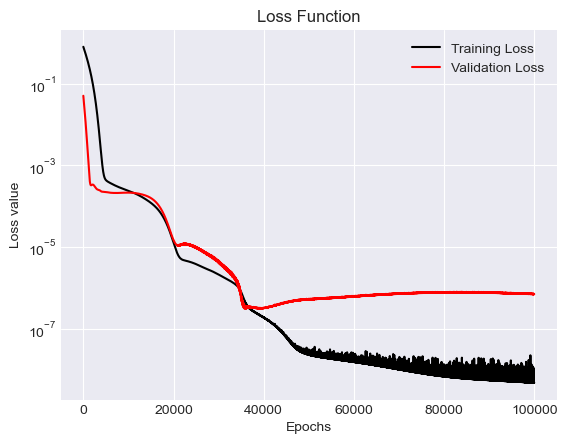
\includegraphics[width=\textwidth]{imgs/error-hernquist.png}
    \caption{Evolution of training and validation error functions as a function of the epoch during the PINN training phase. It can be seen that after about 35,000 epochs, the validation error no longer decreases, or even slightly increases. The training error continues to decrease, a sign of overfitting. The final fluctuations are due to a learning rate too high compared to the error. It should also be noted that what is displayed is the square of the error. A value here of $10^{-6}$ actually corresponds to an absolute error of $10^{-3}$.}
    \label{fig:losses-hernquist}
\end{figure}

Indeed, if the goal is to determine a general solution within a domain, there is no point in infinitely increasing the number of epochs as the validation error no longer decreases. The network is then only over-learning on the collocation points. On the other hand, if the goal is to solve the equation at given points, the number of epochs can be increased until the desired accuracy is reached. This process is time-consuming, but can prove useful in more complex cases than the Hernquist model, as we will see in section~\ref{sec:disk} with the thick exponential disk.

\subsubsection{Results}

The results of the PINN training are explicitly described by Figures~\ref{fig:test-plot-hernquist} and~\ref{fig:relative-error-hernquist}. Using a "light" PINN: $(1 \times 32 + 32)^{(1)} + (32 \times 32 + 32)^{(2)} + (32 \times 1+ 1)^{(3)} = 1153$ parameters\footnote{See Appendix~\ref{app:num-parameters} for details on how to compute the total number of parameters in a network.}, the error obtained is satisfactory, averaging 1.71\%. These results are achieved without performing hyperparameter search and could certainly be improved.

With this result, we can determine the value of the potential at any point in the domain $[0, 1000]$, with great precision, and above all, almost instantly ($1.24$ms $\pm 3.68 \mu $s on an Apple M1 chip). However, if the idea is to \emph{solve} the Poisson equation with the PINN, in the case of the Hernquist potential, it is much more efficient to use traditional methods. For example, the solution is calculated in a few milliseconds using a Runge-Kutta method, compared to nearly a minute for the training of the PINN used here with $50,000$ epochs.

\begin{figure}
    \centering
        \begin{subfigure}[b]{0.49\textwidth}
        \centering
        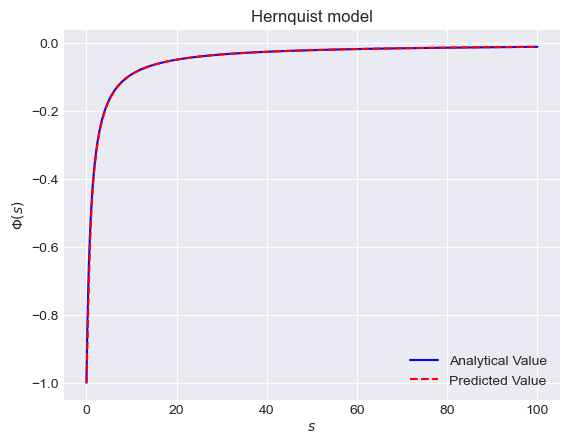
\includegraphics[width=\textwidth]{imgs/test-plot-hernquist.png}
        \caption{Comparison between the actual value of the potential and that predicted by the PINN on a test domain $s \in [0, 100]$.}
        \label{fig:test-plot-hernquist}
        \end{subfigure}
    \hfill
    \begin{subfigure}[b]{0.49\textwidth}
        \centering
        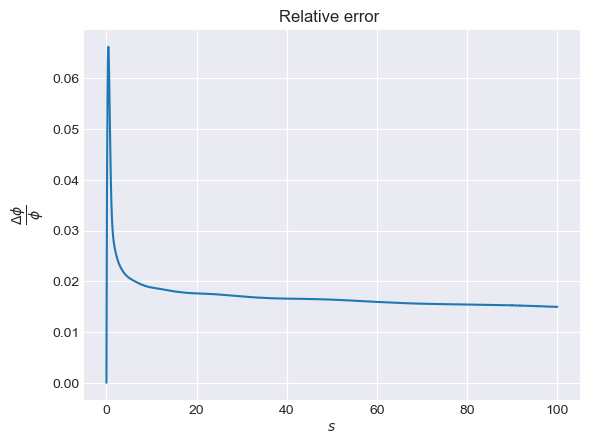
\includegraphics[width=\textwidth]{imgs/relative-error-hernquist.png}
        \caption{Relative error along the domain $s$. The average error over the entire domain is $1.71$\%.}
        \label{fig:relative-error-hernquist}
    \end{subfigure}
    \caption{As illustrated by the two figures presented, a PINN is capable of predicting with acceptable accuracy the value of the Hernquist potential $\Phi$ at a given point in a domain in which it has been trained.}
    \label{fig:three graphs}
\end{figure}

\section{Dehnen Model}\label{sec:dehnen}

In section~\ref{sec:hernquist}, we confirmed the capability of PINNs to solve simple, single-variable problems. With the Dehnen model, we want to verify whether a PINN performs just as well on a multi-parameter model.

\subsubsection{Theory}

We recall the expression of the differential equation~\eqref{eq:poisson-dehnen} that we want to solve in the case of the Dehnen model:

\begin{equation*}
    \dfrac{\dd}{\dd s}\left(s^2 \dfrac{\dd \Phi'}{\dd s}\right) = \dfrac{2s^{2-\gamma}}{(1+s)^{4-\gamma}}
\end{equation*}

A difficulty of this model is the exponent $\gamma$, which drastically changes the dynamics of the potential, as illustrated in Figure~\ref{fig:gamma-vs-x0-dehnen}. During the training of the Hernquist model, it was observed that the PINN was very sensitive to initial conditions. We will discuss this difficulty for the Dehnen model during the generation of training data.

Using equations~\eqref{eq:poisson-dehnen} and~\eqref{eq:loss-galaxy}, we write the error function for this model as follows:

\begin{equation}
    \label{eq:loss-dehnen-explicit}
    \mathcal{L}(\theta) = \dfrac{1}{N_c}\sum^{N_c}_{i=1} \left|\dfrac{\dd}{\dd s_i}\left(s_{i}^{2} \dfrac{\dd \Phi'}{\dd s_i}\right) - \dfrac{2s_i^{2-\gamma}}{(1+s_i)^{4-\gamma}} \right|^2 + \dfrac{1}{N_d}\sum^{N_d}_{i=1} \left|\hat{\Phi}(s_i) - \Phi_i\right|^2
\end{equation}

As shown in the previous example, the implementation of this error function is relatively simple using the PyTorch module. In fact, one of the strengths of the PINN is its adaptability. To move from one model to another, one simply has to modify the function encoding the residual of the PDE, as well as adapt the training points. It is also likely that the hyperparameters of the PINN change from one model to another.

\subsubsection{Training Points}

While for the Hernquist model, we study the potential according to only one parameter, the radius $s$, here we want our PINN to be able to determine the value of the potential according to the radius $s$ and the parameter $\gamma$. Our PINN is therefore a function of two parameters. To handle this, we define the integration domain as being a grid $[s_0, s_n] \times [\gamma_0, \gamma_n]$. While the values of $\gamma$ are dictated by the model, we must choose values for the $s$ interval. Here it is impossible to take $s_0=0$ as equation~\eqref{eq:pot-dehnen} would be undefined in the case where $\gamma \geq 2$. We therefore choose a value of $s_0=10^{-2}$, sufficiently close to $0$. For the choice of $s_n$, we proceed as for the Hernquist case, we want $\Phi(s_n, \gamma) = \varepsilon \approx 0$. However, the behavior of the potential also depends on $\gamma$. The greater the value of $\gamma$, the slower the potential converges to $0$. Therefore, to determine the value of $s_n$, we can set $\gamma = \gamma_n$, and we make sure that the value of $s_n$ found in this case is greater than that corresponding to any other $\gamma_i$. In other words,
\begin{equation*}
    \Phi(s_n, \gamma_0) \leq \Phi(s_n, \gamma_1) \dots \Phi(s_n, \gamma_{n-1}) \leq \Phi(s_n, \gamma_n) = \varepsilon
\end{equation*} It is easy to show that for $\gamma_n = 3 - \delta$, where $\delta \ll 1$,

\begin{align*}
    \label{eq:final-value-hernquist}
    |\Phi(s_n, \gamma_n)| &= -\dfrac{1}{2 - \gamma_n} \left[1 - \left( \dfrac{s_n}{1 + s_n} \right )^{2-\gamma_n}\right] \\
    &= -\dfrac{1}{- 1 + \delta} \left[1 - \left( \dfrac{s_n}{1 + s_n} \right )^{- 1 + \delta}\right] \\
    &= -\dfrac{1}{- 1 + \delta} \left[1 - \left( \dfrac{1 + s_n}{s_n} \right )^{1 - \delta}\right] \\
    &\approx -\dfrac{1}{- 1} \left[1 - \left( \dfrac{1 + s_n}{s_n} \right )^{1}\right]\\
    &\approx \left[1 - \left( \dfrac{1}{s_n} + 1 \right )\right]\\
    &\approx - \dfrac{1}{s_n}\\
    \Rightarrow |s_n| &= \frac{1}{\varepsilon}
\end{align*} Thus, if we wish to have $\varepsilon=10^{-3}$ as before, we can choose $s_n=1000$. Consequently, the integration is done on the domain $[0.01, 1000] \times [0, 3[$. We proceed in the same way as before to select the training and validation points, as illustrated on Figure~\ref{fig:aberration-dehnen}. A major difference with the Hernquist case is the number of collocation points and data points. In fact, we had chosen $N_c=1024$ for the Hernquist profile, and $N_d=2$ was imposed on us by the only two boundaries of the domain. Now that we have a grid, we can freely choose the value of $N_d$.
\par We want to sufficiently cover the boundaries, especially the one at $s=0$, for which the PINN is particularly sensitive. To avoid increasing the computation time too much, we first choose $N_d=512$. Regarding the collocation points, we had $N_c=1024$ in one dimension. Proceeding with the same number of points per dimension would be too time-consuming. Therefore, instead of selecting $N_c=1024^2 \approx 10^6$, we start with $N_c=8192$. We will discuss the influence of these collocation and data points when presenting the results.

\begin{figure}
\centering
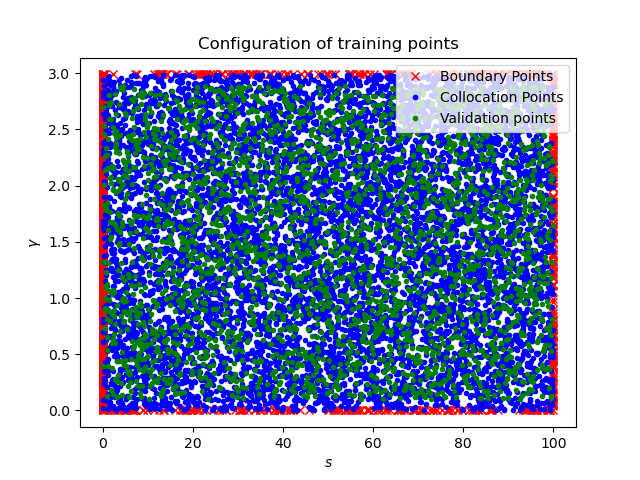
\includegraphics[width=\textwidth]{imgs/training-points-dehnen.png}
\caption{Distribution of training and validation points on the domain.}
\label{fig:training-points-dehnen}
\end{figure}

\subsubsection{Training}

The Dehnen profile presents more complex characteristics than the Hernquist one. This is particularly due to the large dynamic range caused by the $\gamma$ exponent, as illustrated in Figure~\ref{fig:gamma-vs-x0-dehnen}. The previously used architecture is not able to learn this dynamic, and thus fails to recover the gravitational potential with a satisfactory error.

\begin{figure}
\centering
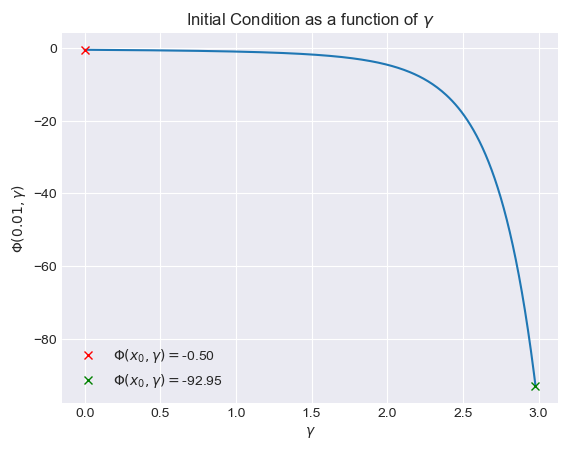
\includegraphics[width=\textwidth]{imgs/gamma-vs-x0-dehnen.png}
\caption{Value of the gravitational potential at $s_0 = 0.01$ for different values of $\gamma \in [0, 3[$. Predicting the potential value at $s_0=0$ is a complex task for the PINN given the high sensitivity of $\Phi(s_0, \gamma)$ to the value of $\gamma$.}
\label{fig:gamma-vs-x0-dehnen}
\end{figure}

\par Several parameters were tested manually, including the number of collocation and data points, the network architecture, the learning rate, and the error type. Finding parameters that provide acceptable accuracy was a complex task. While the learning rate only slightly changes the final result (for reasonable variations of this rate), the results vary extremely with the other parameters. Particularly, for a certain architecture, one can go from a correct solution to an aberrant one depending on the chosen number of points $N_c$ and $N_d$. It also appears that if the total number of neurons in the network is high, but there are too few collocation points, the PINN seems to overfit these points. We then obtain totally false results, as illustrated in Figure~\ref{fig:aberration-dehnen}.

\begin{figure}
    \centering
    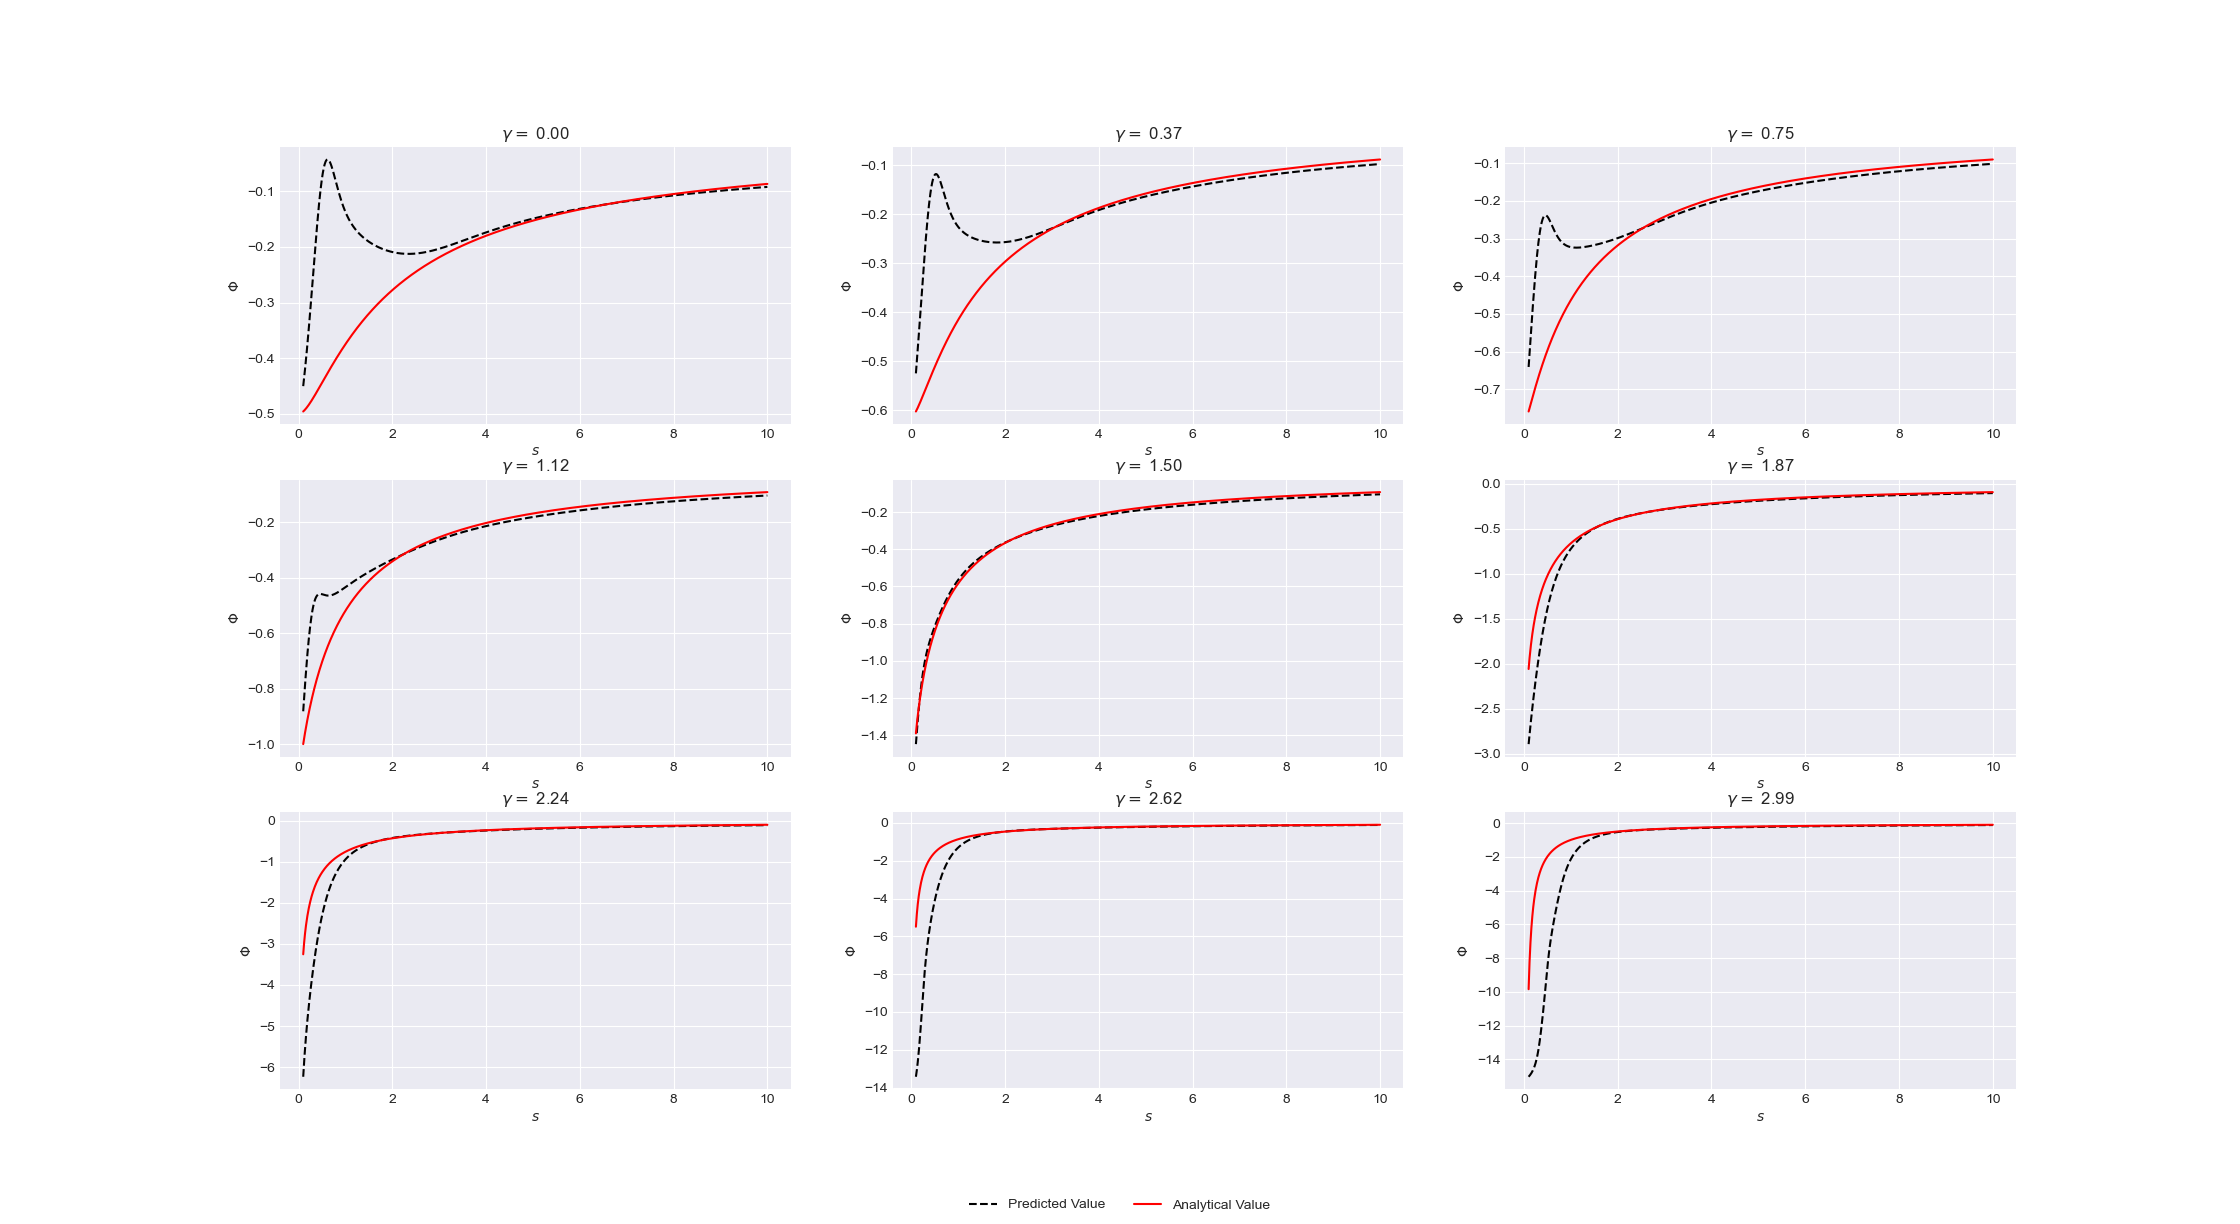
\includegraphics[width=\textwidth]{imgs/aberration-dehnen.png}
    \caption{Outlying results obtained for $N_d=100$, $N_c=1024$ and an architecture of two layers of 32 neurons.}
    \label{fig:aberration-dehnen}
\end{figure}

Most of the trials have shown that only certain parts of the domain were misunderstood, and that others were in almost perfect agreement with the real solution, a phenomenon well illustrated by Figure~\ref{fig:aberration-dehnen}. For small values of $s$ (between 0 and about $s_n/10$), and $\gamma \geq 2$, predictions are often wrong, resulting in high penalty due to the quadratic error. However, this penalty is compensated by the very small values of the quadratic error over the rest of the domain, where the prediction is in good agreement with the real value. One idea is to modify the penalty function so that the contribution of large errors is better taken into account. Ideally, a problem-specific penalty function that would depend on $\gamma$ would be most suitable, but we have found that the mean absolute error (MAE) penalty gives satisfactory results. We define the mean absolute error as follows:

\begin{equation}
\label{eq:mae}
    MAE = \frac{1}{N}\sum_{i=1}^{N} \left| \hat{\Phi}(s_i) - \Phi_i\right|
\end{equation}

\subsubsection{Results}

Despite the fact that the network can see all the initial points thanks to the data points distributed on the left border, it does not manage to correctly reproduce the potential for small values of $s$ and large values of $\gamma$ (see Figures~\ref{fig:relative-error-dehnen} and~\ref{fig:test-plot-dehnen}). By changing the penalty to quantify the error, we have been able to achieve good results for a simple network comprising a hidden layer of 32 neurons and another one of 16, using a tanh activation function. Contrary to what we thought, a simple architecture has been able to determine the potential with an accuracy of about 4\%. Perhaps even more surprisingly, using fewer training points proved to be more effective in reducing the error. Thus, the best result obtained, without hyperparameter search, was achieved with $N_c = 1024$ and $N_d=100$. To avoid degrading the resolution with this small number of points, we reduced the value of $s_n$ and finally took an integration domain $s \in [0, 10]$, with $300\times50$ points from which the collocation points are selected. As previously noted, there is an unclear link between the number of neurons in the network and the number of points used. In general, the influence and correlations between the hyperparameters for the Dehnen case is rather poorly understood. This interpretability of the PINN is one of the axes of progress of this work, as will be discussed in Chapter~\ref{ch:conclusion}.

The result is here less clear than for the Hernquist model. It is possible for us to determine the value of the potential at any point in the domain $[0, 10] \times [0, 3[$ with a very variable accuracy; error ranging from less than 1\% to about 20\% depending on the region (see Figure~\ref{fig:relative-error-dehnen}). However, with very little effort--the implementation of a residual function for the Dehnen profile--it is possible to have an estimate of the potential on a whole grid almost instantaneously. Training the model itself only takes a few seconds, thanks notably to the small size of the network used and the few points used. For a more complicated profile, without an analytical solution, a PINN with similar results could be used for a parameter search. The average error of 3.75\% is probably small enough to distinguish between different cases. We thus show that a PINN, provided it is equipped with the right hyperparameters, can determine the equation of a parametrized potential with an error of the order of a few percent only.

\begin{figure}
    \centering
    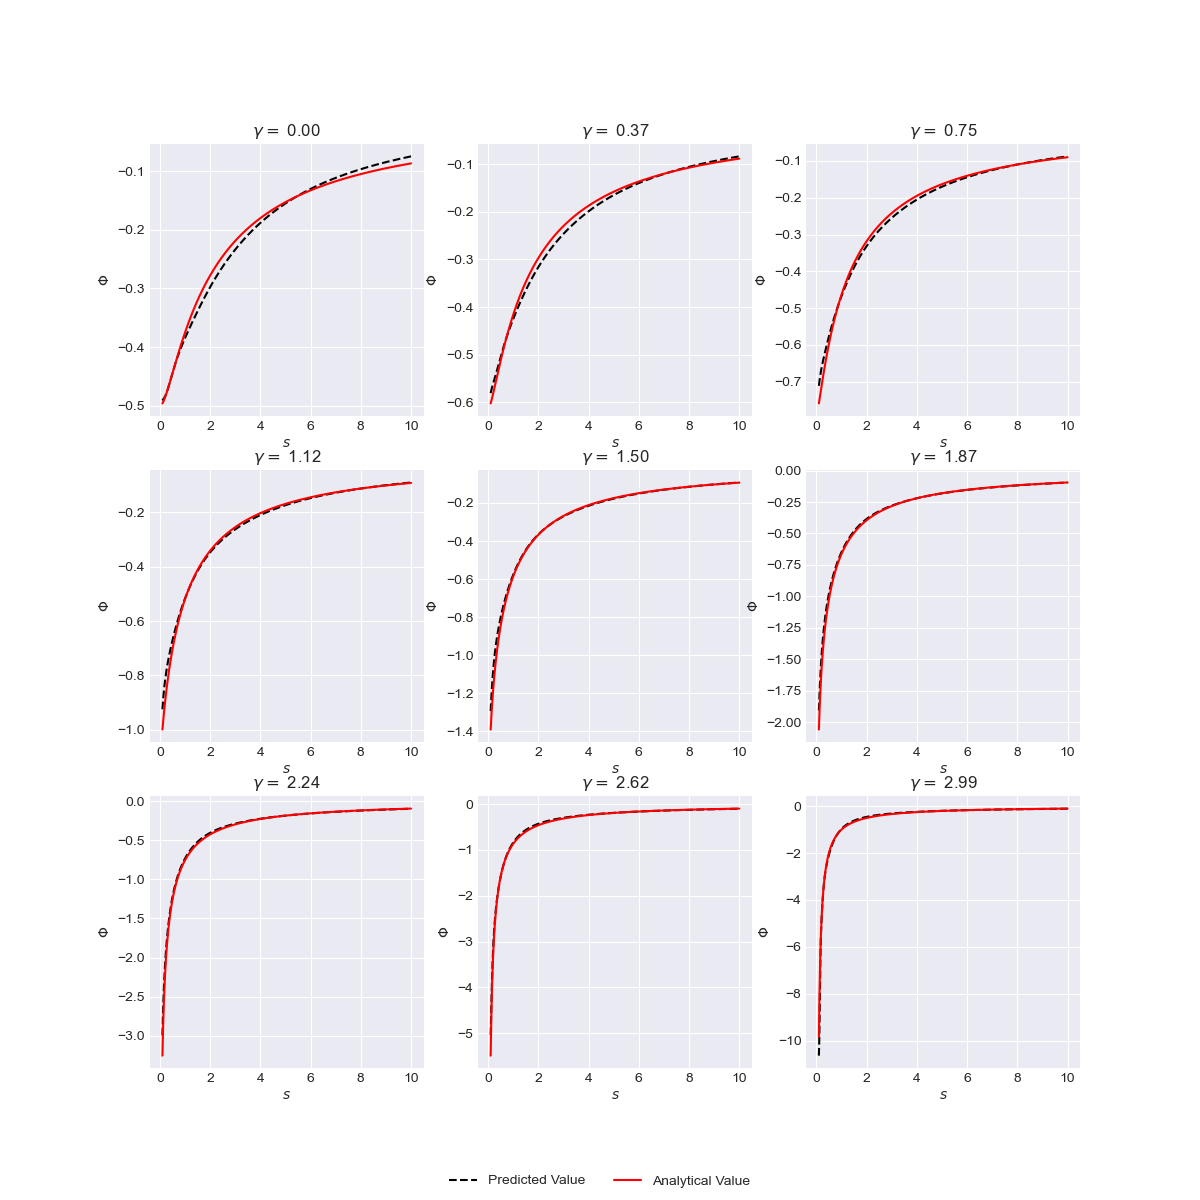
\includegraphics[width=\textwidth]{imgs/test-plot-dehnen.png}
    \caption{Comparison between the real value of the potential and that predicted by the PINN on a test domain $s \in [0, 10]$ for different values of $\gamma$.}
    \label{fig:test-plot-dehnen}
\end{figure}

\begin{figure}
    \centering
    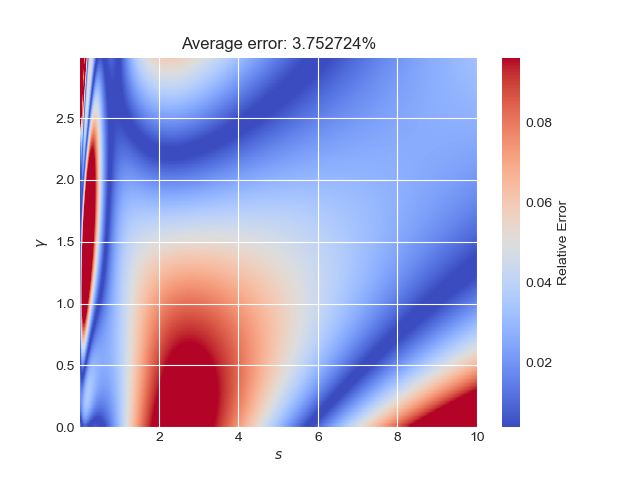
\includegraphics[width=\textwidth]{imgs/relative-error-dehnen.png}
    \caption{Relative error on the $s \times \gamma$ grid. The average error over the entire domain is 3.75\%. It is noted that certain parts of the grid are not well understood by the PINN. The relative error reaches nearly 20\% there.}
    \label{fig:relative-error-dehnen}
\end{figure}

\section{Thick Exponential Disk}\label{sec:disk}

With the Hernquist and Dehnen models, we demonstrated the ability of PINNs to solve the gravitational Poisson equation for radial densities. With the thick exponential disk model, we now want to check the ability of PINNs to understand axisymmetric models, which more faithfully describe real systems.

\subsubsection{Theory}
\par We recall the differential equation~\eqref{eq:poisson-exp-disc-final} that we want to solve:

\begin{equation}
\label{eq:residu-poisson-2}
\dfrac{1}{R'} \dfrac{\partial}{\partial R'} \left(R' \dfrac{\partial \Phi'}{\partial R'}\right) + \dfrac{1}{\eta^{2}}\dfrac{\partial^2 \Phi'}{\partial z'^2} = e^{-R'} \cosh^{-2}{z'}
\end{equation} Similarly to what we did for the Hernquist and Dehnen models, we use this equation along with the definition of the loss function~\eqref{eq:loss-galaxy} to formulate the loss function specific to our problem:

\begin{equation}
    \label{eq:loss-func-hernquist}
    \begin{aligned}
        \mathcal{L}(\theta) &= \dfrac{1}{N_c}\sum^{N_c}_{i=1} \left\|\dfrac{1}{R'_i} \dfrac{\partial}{\partial R'_i} \left(R'_i \dfrac{\partial \Phi'}{\partial R'_i}\right) + \dfrac{1}{\eta^{2}}\dfrac{\partial^2 \Phi'}{\partial z_{i}^{'2}} - e^{-R'_i} \cosh^{-2}{z'_i} \right\|^2 \\
        &+ \dfrac{1}{N_d}\sum^{N_d}_{i=1} \left\|\hat{\Phi}(R'_i, z'_i) - \Phi_i \right\|^2
    \end{aligned}
\end{equation}  Similar to the Dehnen case, the PINN here is a function of several parameters; $R'$, $z'$ and $\eta$. In the context of this work, we fix $\eta$, and let the PINN be a function of only two parameters. As with the Dehnen model, we will place the data and collocation points on a grid.

\subsubsection{Training Points}

Here, we wish to use precise values for the parameters. Thus, we set $\eta=0.2$, $R_d=4$, and thus $z_d=0.8$. Moreover, we wish for our integration domain $R' = \frac{R}{R_d} =[0, 20]$ and $z'= \frac{z}{z_d} =[0, 5]$. We create a $R' \times z'$ grid composed of $250 \times 250$ points, among which we select using the Latin hypercube sampling algorithm $N_c=1024$ collocation points. Using the same method, we select $N_d=296$ data points located on the domain boundaries. For the latter, more work was needed compared to the previous cases. We first needed to be able to know the value of the potential at the selected border points. To do this, we first simulated the gravitational potential of the disk with the aforementioned parameters, and a grid of $250\times250$ points. This was done by integrating equation~\eqref{eq:exp-disk-potential} using the Python interface of QUADPACK provided by the Scipy library~\cite{2020SciPy-NMeth}. Then, we performed linear interpolation on the grid $[0, 20] \times [0, 5]$. The selected points are illustrated in Figure~\ref{fig:training-points-expdisc}, along with the validation points.

\begin{figure}
\centering
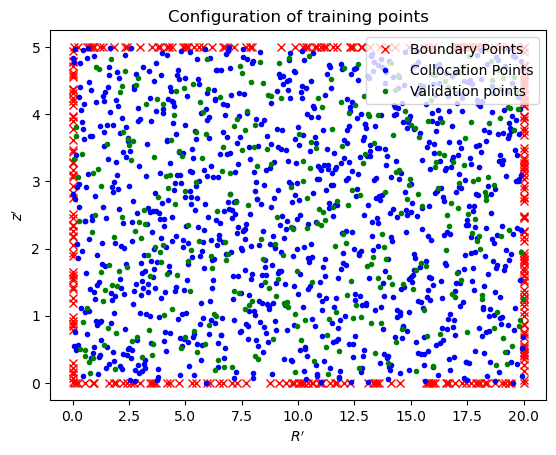
\includegraphics[width=\textwidth]{imgs/training-points-expdisc.png}
\caption{Distribution of training and validation points on the domain $[0, 20] \times [0, 5]$.}
\label{fig:training-points-expdisc}
\end{figure}

\subsubsection{Training}

The motivations behind training the thick exponential disk model are somewhat different than in the previous two cases. Indeed, the previous two models admitted analytical solutions, and using a PINN to describe their potential ultimately had no practical interest. In these two cases, the use of a PINN was solely a proof of concept. For the thick exponential disk, however, being able to predict the potential on an entire grid almost instantly is of real interest. We strive here to minimize the error made during this prediction as much as possible. Thus, once the PINN's ability to solve the potential in the case of the thick exponential disk has been attested with a simple network, we set out to fine-tune the hyperparameters. These two searches have shown interesting results for different reasons.

For the fine-tuning of the hyperparameters, we conducted a simple grid search on the parameters presented in Table~\ref{tab:fine-tuning}. The models were compared using the average relative error obtained on a validation data set. This search allows in particular to study the influence of hyperparameters on the average relative error. We also controlled the median value, the minimum and maximum of the relative error, which we will not however exploit in this succinct analysis.

\begin{table}[h]
\centering
\begin{tabular}{|l|c|}
\hline
\textbf{Parameters} & \textbf{Values} \\
    \hline
    \# Neurons & 32, 64, 128 \\
    \hline
    \# Layers & 1, 2, 3, 4, 5, 6 \\
    \hline
    Learning Rate & 1e-4, 1e-5, 1e-6 \\
    \hline
    Loss Func. & mse \\
    \hline
    Activation & Tanh, Sigmoid, SiLU, LogSigmoid \\
    \hline
\end{tabular}
\caption{List of hyperparameters tested during the grid search. We tested, for example, networks with 32, 64 or 128 neurons per layer and, with one to six hidden layers. For the loss function, we limited ourselves to the mean squared error to limit computation time. In total, 216 networks with different combinations were tested, each trained over 10,000 epochs.}
\label{tab:fine-tuning}
\end{table} With an average relative error of 0.09\%, the model with an architecture of 6 hidden layers of 64 neurons, a sigmoid activation function and a learning rate of $10^{-6}$ is the one giving the best results. However, we prefer to ensure that we have a robust model, which does not have any aberrant points. We instead choose the model with the lowest maximum relative error, i.e., the place on the grid with the largest error. With a maximum relative error of 0.13\%, this model uses a tanh activation function, an architecture of 6 hidden layers of 128 neurons and, a learning rate of $10^{-6}$. We finally train this network for $50,000$ epochs.

\subsubsection{Results}

First, we present the training performed to test the PINN. We used a network consisting of three hidden layers of 32 neurons each, 30,000 epochs, an Adam optimizer, a learning rate of $10^{-4}$, and a tanh activation function. In about 87 seconds of training, the PINN, with the aforementioned hyperparameters, determines the potential over the entire grid. The achieved accuracy is satisfactory, with an average relative error of $1.85\%$ and a maximum of $5.88\%$. This result is interesting in practice as even using the highly optimized Scipy interface, the solution is computed in about 8min 11s, on the same computer. This is about $5.6\times$ slower. Moreover, this solution with Scipy was reached using as integration limits $a=0$, $b=200$, the maximum value of $b$ for which equation~\eqref{eq:hypergeometric} remains defined when the argument $z=-e^{s\beta}$. To circumvent this problem we tried other implementations of the Gauss hypergeometric function, but the computing time exploded and took several days. In sum, the PINN offers an easy and quick solution to implement a solver for the thick exponential disk potential.

On the other hand, using the fine-tuned PINN, we are able to determine the potential over the entire domain $[0, 20] \times [0, 5]$ and all subdomains with an average accuracy of 0.36\%. The results over the entire grid are shown in Figure~\ref{fig:relative-error-expdisc}. Training for such a deep network takes about 20 minutes. However, once trained the potential can be determined at any point on the grid in a few milliseconds. To be able to determine the best parameters for a system modeled as a thick exponential disk, it would now be necessary to extend the PINN so that it can take the parameter $\eta$ as an argument.

\begin{figure}
\centering
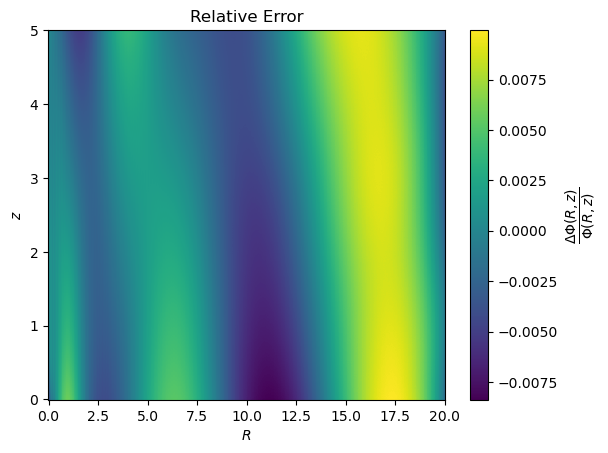
\includegraphics[width=\textwidth]{imgs/relative-error-expdisc.png}
\caption{Relative error on the $R' \times z'$ grid. The average error over the entire domain is 0.36\%, and the maximum error is 0.99\%.}
\label{fig:relative-error-expdisc}
\end{figure}

Beyond the ability of a PINN to solve equation~\eqref{eq:poisson-exp-disc-final} with high precision, this analysis also yielded results on the influence of the model's hyperparameters. We briefly discuss these results here, particularly illustrated by Figures~\ref{fig:function-error-expdisc} to~\ref{fig:layers-error-expdisc}. It is quite clear that the tanh function gives on average the smallest error, and that a low learning rate is also associated with a lower error. The analysis regarding the number of neurons and hidden layers is less evident. Several effects are observable. First of all, we notice in Figure~\ref{fig:neurons-error-expdisc} that the error reduction between 64 and 128 neurons is relatively small compared to the decrease observed when moving from 32 to 64 neurons per layer. Unfortunately, no definitive conclusion can be drawn with so few data points, but it seems that accuracy saturates at some point with the width of the network. In other words, increasing the width of the network -- the number of neurons per layer -- may not have as much influence as the depth of the network. Indeed, accuracy seems to improve more regularly with the number of hidden layers used (see Figure~\ref{fig:layers-error-expdisc}). One must keep in mind the variation in the total number of neurons in the network. Does the relative error only decrease based on the number of neurons used, or does the architecture -- the arrangement of these neurons -- also play a role? We notice on Figure~\ref{fig:tot-neurons-error} that the relative error is not simply proportional to the total number of neurons present in the PINN. This indicates that the architecture has an effect on the error.

With the help of Table~\ref{table:total_neurons}, we can link the architectures to the total number of neurons indicated on Figure~\ref{fig:tot-neurons-error}. We particularly note that on average the PINNs with 320 neurons, corresponding to an architecture of 5 hidden layers and 64 neurons per layers, are those giving the smallest relative error. It is not yet well understood how depth or width influences the accuracy of the PINN.

\begin{figure}
\centering
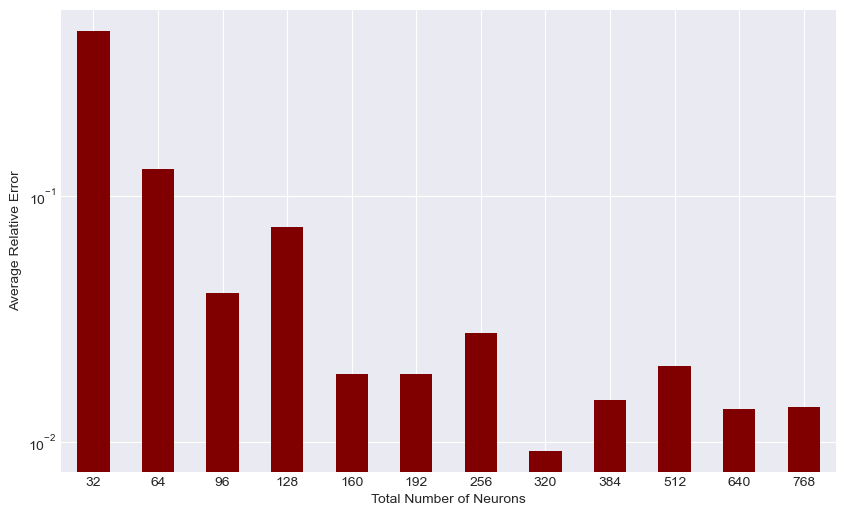
\includegraphics[width=\textwidth]{imgs/tot-neurons-error.png}
\caption{Evolution of the average relative error as a function of the total number of neurons in the PINNs.}
\label{fig:tot-neurons-error}
\end{figure}

\begin{table}
\centering
\begin{tabular}{|c|c|c|c|}
    \hline
     & \textbf{32} & \textbf{64} & \textbf{128} \\
    \hline
    \textbf{1}  & 32 & 64 & 128 \\
    \hline
    \textbf{2}  & 64 & 128 & 256 \\
    \hline
    \textbf{3}  & 96 & 192 & 384 \\
    \hline
    \textbf{4}  & 128 & 256 & 512 \\
    \hline
    \textbf{5}  & 160 & 320 & 640 \\
    \hline
    \textbf{6}  & 192 & 384 & 768 \\
    \hline
\end{tabular}
\caption{Total number of neurons for a given number of neurons per layer and a given number of layers. The number of hidden layers, ranging from 1 to 6, is given at the start of each row. The number of neurons per hidden layer is given at the start of each column.}
\label{table:total_neurons}
\end{table}

\begin{sidewaysfigure}
\centering
\begin{subfigure}{.5\textwidth}
\centering
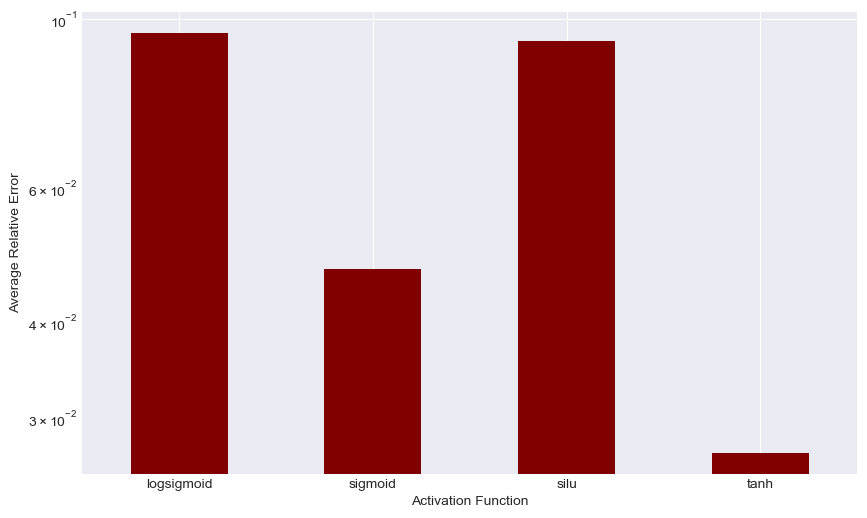
\includegraphics[width=1\linewidth]{imgs/function-error-expdisc.png}
\caption{Average relative error for certain activation functions.}
\label{fig:function-error-expdisc}
\end{subfigure}%
\begin{subfigure}{.5\textwidth}
\centering
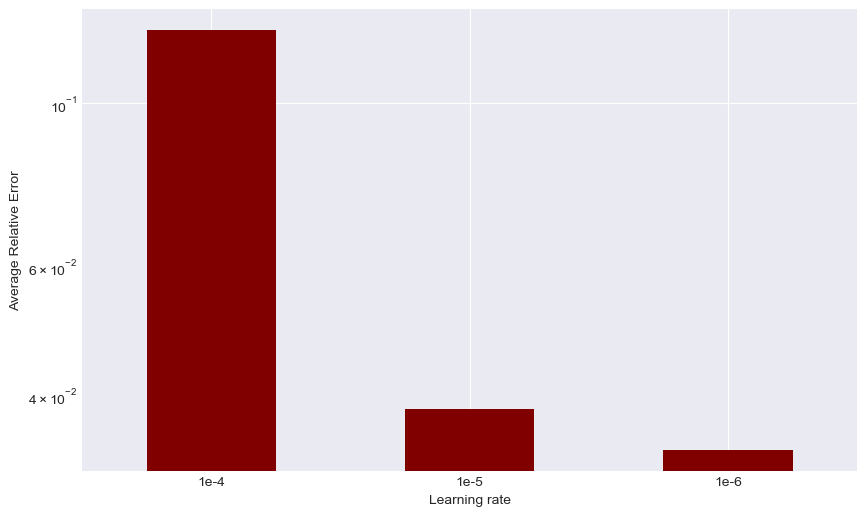
\includegraphics[width=1\linewidth]{imgs/learning-rate-expdisc.png}
\caption{Average relative error for different learning rates.}
\label{fig:learning-rate-expdisc}
\end{subfigure}
\begin{subfigure}{.5\textwidth}
\centering
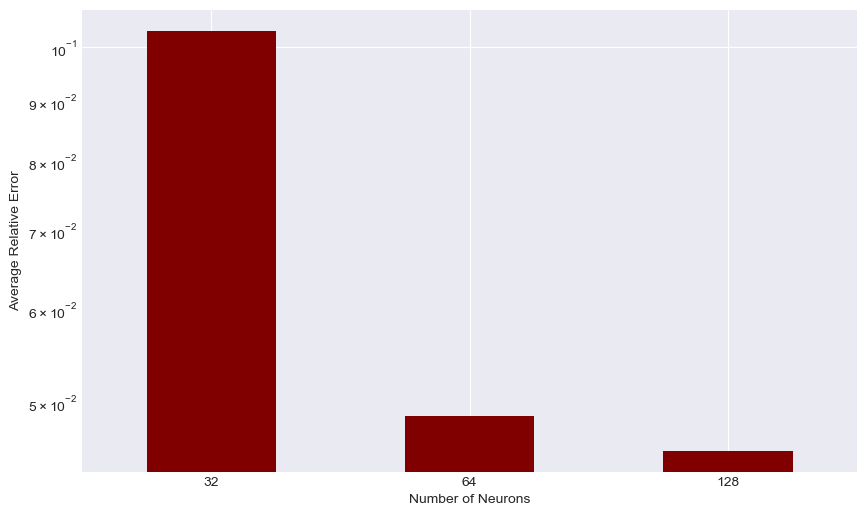
\includegraphics[width=1\linewidth]{imgs/neurons-error-expdisc.png}
\caption{Influence of the number of neurons per hidden layer on the average relative error.}
\label{fig:neurons-error-expdisc}
\end{subfigure}%
\begin{subfigure}{.5\textwidth}
\centering
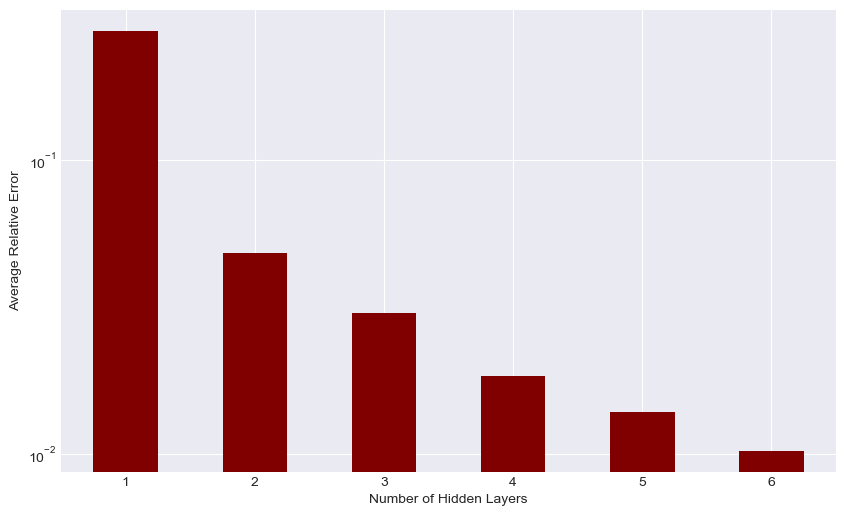
\includegraphics[width=1\linewidth]{imgs/layers-error-expdisc.png}
\caption{Influence of the number of hidden layers on the average relative error.}
\label{fig:layers-error-expdisc}
\end{subfigure}
\caption{Evolution of the average relative error depending on the hyperparameters tested during the grid search. Notably, we can see that the tanh function produces on average the smallest average relative error, or that it is much more preferable to choose 64 or 128 neurons per layer rather than 32.}
\label{fig:hyperparametres-vs-error}
\end{sidewaysfigure}